\chapter{Apêndice A}
\label{appendixA}

\section{Modelos Estudados}

\subsection{Marigold}

Os autores \cite{ke2024repurposing} apresentaram o Marigold, um modelo de difusão latente baseado em \textit{Stable Diffusion} (SD). Modelos fundacionais de visão computacional, como o SD, são treinados com dados em larga escala e em uma vasta gama de domínios. O seu funcionamento e baseado na premissa de que a tarefa de MDE possui como pilar a plena compreensão das representações visuais do mundo, portanto, é possível aproveitar o conhecimento prévio de um modelo fundacional de difusão para transforma-lo em um estimador de profundidade. Desse modo é proposto um protocolo de ajuste fino (ou do inglês, \textit{fine-tuning}) que objetiva a adaptação de um modelo de difusão latente para um modelo de MDE, mostrado na Figura \ref{marifino}.

\begin{figure}[h]
    \centering
    \caption{Protocolo de ajuste fino do Marigold.}
    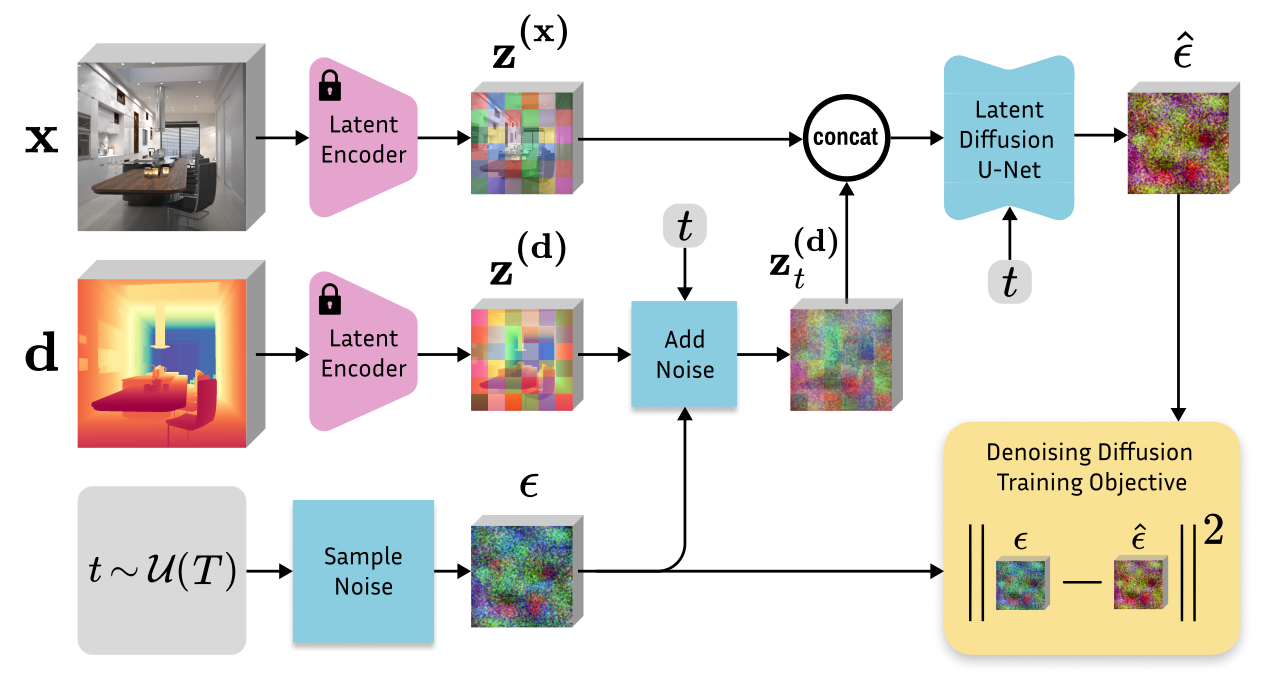
\includegraphics[width=.8\textwidth]{fig/mariouro.png}
    \caption*{Fonte: \citeonline{ke2024repurposing}}
    \label{marifino}
\end{figure}

Um VAE (\textit{Variational Auto Encoder}) pré-treinado, proveniente do SD, é empregado para projetar a imagem RGB e o mapa de profundidade em um espaço latente de menor dimensionalidade. O processo de ajuste fino se concentra na componente U-Net, otimizando uma função objetivo. Essa função compara o código latente obtido a partir do ruído de difusão com a representação latente gerada pela U-Net após o processo de remoção de ruído (\textit{denoising}). É importante destacar que apenas os parâmetros da U-Net são ajustados durante o treinamento. 

O processo de inferência funciona de acordo com a Figura \ref{mariinfe}. Dado uma imagem RGB de entrada, ela é processada com por meio do mesmo VAE utilizado no \textit{fine-tuning}) e concatenada com o ruído já no espaço latente. Em seguida, passa pela U-Net para remover o ruído a cada iteração. Depois da execução de $T$ passos de difusão, a imagem é descodificada pelo VAE em uma imagem de 3 canais, que representa o mapa de profundidade final. 

\begin{figure}[h]
    \centering
    \caption{Processo de inferência do Marigold.}
    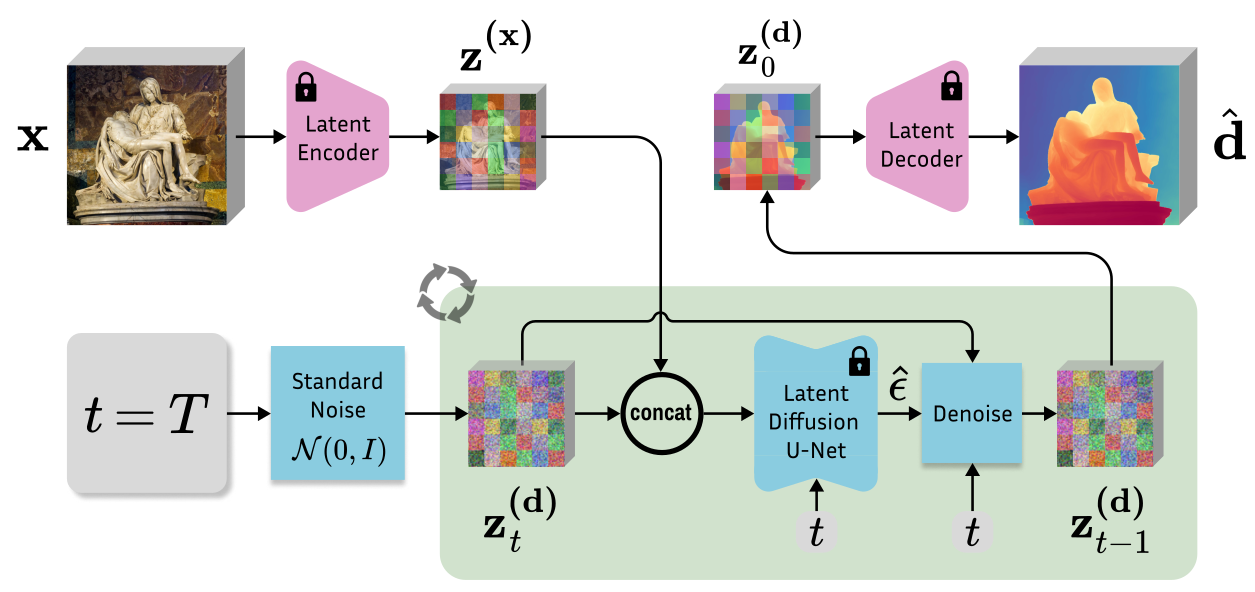
\includegraphics[width=.8\textwidth]{fig/mariouro2.png}
    \caption*{Fonte: \citeonline{ke2024repurposing}}
    \label{mariinfe}
\end{figure}